\documentclass[11pt,a4paper]{article}
\usepackage{ucs}
\usepackage[T1]{fontenc}
\usepackage[utf8x]{inputenc}
\usepackage[german]{babel}
\usepackage{amsmath}
\usepackage{amsfonts}
\usepackage{amssymb}
\usepackage{graphicx}
\usepackage{shadethm}
\usepackage{caption}
\usepackage{tikz} 



\newshadetheorem{sdefinition}{Definition}
\newenvironment{definition}[1][]{%
  \definecolor{shadethmcolor}{rgb}{1.0,1.0,1.0}%{.9,.9,.9}%
  \definecolor{shaderulecolor}{rgb}{0.0,0.0,0.0}%
  \setlength{\shadeboxrule}{1pt}%
  \begin{sdefinition}[#1]%
}{\end{sdefinition}}

\newcommand{\minipanf}{\begin{minipage}{\linewidth}}
\newcommand{\minipend}{\end{minipage}}

\begin{document}

\begin{titlepage}
\newcommand{\HRule}{\rule{\linewidth}{0.5mm}} % Defines a new command for the horizontal lines, change thickness here

\center % Center everything on the page
 
%----------------------------------------------------------------------------------------
%	HEADING SECTIONS
%----------------------------------------------------------------------------------------

\textsc{\LARGE TU Dresden}\\[1.5cm] % Name of your university/college
\textsc{\Large Fortgeschrittenenpraktikum}\\[0.5cm] % Major heading such as course name
\textsc{\Large Praktikumsbericht}\\[0.5cm] % Major heading such as course name

%----------------------------------------------------------------------------------------
%	TITLE SECTION
%----------------------------------------------------------------------------------------

\HRule \\[0.7cm]
{ \huge \bfseries Dosimetrie}\\[0.4cm] % Title of your document
\HRule \\[1.5cm]
 
%----------------------------------------------------------------------------------------
%	AUTHOR SECTION
%----------------------------------------------------------------------------------------

\begin{minipage}{0.4\textwidth}
\begin{flushleft} \large
\emph{Autoren:}\\
Toni \textsc{Ehmcke}\\
Christian \textsc{Siegel}
\end{flushleft}
\end{minipage}
~
\begin{minipage}{0.4\textwidth}
\begin{flushright} \large
\emph{Betreuer:} \\
Birgit \textsc{Schneider} % Supervisor's Name
\end{flushright}
\end{minipage}\\[4cm]

%----------------------------------------------------------------------------------------
%	DATE SECTION
%----------------------------------------------------------------------------------------

{\large Dresden, \today}\\[3cm] % Date, change the \today to a set date if you want to be precise

\vfill 

\end{titlepage} 	% Titelseite

\tableofcontents

\section{Aufgabenstellung}
Im Experiment werden wir die folgenden Aufgabenstellungen bearbeiten:
\subsection{Strahlenschutzkontrollmessungen}
Zunächst bestimmen wir die Dosisleistung in den Bestrahlungsräumen bei geschlossener und geöffneter Quelle an Positionen, an denen später gemessen wird und an denen wir uns häufig aufhalten werden. Dies hat den Zweck der Überwachung der durch die Experimentatoren aufgenommenen Dosis und des Strahlungshintergrundes, welcher die spätere Dosismessung beeinflussen kann. Es soll eine Skizze des Messraumes mit den entsprechenden Dosiswerten entstehen.

\subsection{Winkelabhängigkeit einer Ionisationskammer}
Mit Hilfe einer Stielkammer ($V = 30,0\ cm^3$) soll die Richtungsabhängigkeit der Ionisationskammer bei einem festem Abstand ($d=0.5\ m$) und variablem Azimutalwinkel $\phi$ untersucht werden.
Dies dient der Ermittlung der optimalen Ausrichtung der Kammer zur Bestimmung der Referenzdosisleistung für die spätere OSL-Dosimetrie.

\subsection{Abschätzung der Dosisleistung für $\gamma$-Strahler}
Für eine $^{137}Cs$-Quelle soll die Dosisleistung für festen Abstand ($d=0.5\ m$) und unter dem oben ermittelten Winkel $\phi$ als Referenzdosis bestimmt werden. Dabei kann

\begin{equation} \label{eq:dosisleistung}
	\dot{D}=\frac{A \cdot \Gamma}{d^2}
\end{equation}
abgeschätzt werden. Dabei sind:
\begin{center}
	\begin{minipage}{.9\textwidth}
		d: Abstand zur Quelle\\
		A: Aktivität der Quelle am Versuchstag(22.10.2015), \\
		Referenzwert $A(27.02.2008) = 5,0\ GBq \equiv A_0$\\
		$\Gamma$: Dosisleistungskonstante
	
	%----------------------------------------Tabelle einfügen---------------------------------
	\end{minipage}
\end{center}

\subsection{Dosismessung mit BeO$max$ und Abstandsquadratsgesetz}
Wir werden anschließend mit Hilfe des BeO\textit{max}-OSL-Dosimetriesystems eine Dosismessung vornehmen. Da dieses Messsystem ein relatives Vorgehen verlangt, wird die Messung in zwei Schritten vorgenommen: 1) der Kalibrierung mit einer bekannten Dosis ($d=0.5\ m$) durch Ermittlung des Ansprechvermögens $\epsilon$ und 2) der Dosisbestimmung einer unbekannten Dosis ($d$ variabel). Dabei untersuchen wir gleichzeitig die Gültigkeit des Abstandsquadratsgesetzes.

\subsection{Winkelabhängigkeit der kollimierten Quelle}
Wir haben bei diesem Versuch eine kollimierte $^{137}Cs$-Quelle verwendet. Dabei werden wir die Abhängigkeit der Dosisleistung vom senkrechten Abstand zum Strahlmittelpunkt bestimmen.
		% Aufgabenstellung
\section{Physikalischer Hintergrund}
\subsection{Dosisgrößen}
Wir definieren nun die wesentlichen Größen zur Charakterisierung der Wechselwirkung/Schädigung von Materie mit ionisierender Strahlung:\\
Die \underline{Dosis D} ist ein Maß des Energieübertrags $\mathrm{d}E$ ionisierender Strahlung auf ein Materie-Massenelement $\mathrm{d}m$:
\begin{equation}\label{eq:dosis}
	D = \frac{\mathrm{d}E}{\mathrm{d}m},\ [D] = J/kg \equiv Gy\ \textrm{(Gray)}
\end{equation}
Die zeitliche Änderung der Dosis $\dot{D}$ nennt man \underline{Dosisleistung}.\\
Will man berücksichtigen, dass die Schädigung biologischen Gewebes sowohl von der Strahlungsart R als auch von der Gewebeart T abhängt, führt man die Wichtungsfaktoren $w_R$ und $w_T$ ein, um die für den Strahlenschutz wesentliche Messgröße der \underline{effektiven (Äquivalent-)Dosis $H_E$} zu definieren:
\begin{equation}
	H_E = \sum_{R,T} w_R \cdot w_T \cdot D_{R,T},\ [H_E]=J/kg \equiv Sv\ \textrm{(Sievert)}
\end{equation}
Dabei findet man, dass die Dosisleistung einer Punktquelle mit dem Quadrat des Abstandes zu dieser fällt:
\begin{equation*}
		\dot{D} \propto \frac{1}{d^2}
\end{equation*}
Diesen Zusammenhang nennt man \textbf{Abstandsquadratgesetz}.\cite{PA_neu}

\subsection{Aktivität}
Um die Dosisleistung für die gegebenen $\gamma$-Strahler in Aufgabe 2.3 abzuschätzen, benötigen wir die \underline{Aktivität A} als Maß für die Anzahl der spontanen Kernumwandlungen pro Zeiteinheit. Mit dem exponentiellen Zerfallsgesetz erhalten wir:
\begin{equation} \label{eq:aktivitaet}
	A(t)=A(t=0) \cdot \left(\frac{1}{2}\right)^{\frac{t}{T_{1/2}}}, [A] = 1/s \equiv Bq \textrm{(Bequerel)}
\end{equation}
Hier bei ist $T_{1/2}$ die Halbwertszeit des gegebenen Isotops.\cite{PA_RM1}

\subsection{Messprinzip: Ionisationskammer}
Grob gesprochen ist eine Ionisationskammer ein (beliebig geformter) Kondensator, dessen Dielektrikum gasförmig (in unserem Fall Luft) vorliegt. Tritt ionisierende Strahlung (Primärteilchen) in das Kammervolumen, so entstehen durch Wechselwirkung - in unserem Falle durch inkohärente Streuung und Photoeffekt - mit den Gasteilchen Elektronen-Ionen-Paare (Sekundärteilchen), indem die Elektronen aus der Atomhülle des bindenden Atoms herausgeschlagen werden. Diese Ladungsträger gelangen nun im Idealfall durch Coulomb-Wechselwirkung zu einer Kondensatorplatte, wo sie nun als Stromfluss I nachgewiesen werden können. Für näherungsweise konstante Dosisleistungen im Zeitintervall $\Delta t$ erhalten wir die Proportionalität zwischen dem Stromfluss und der Dosis:

\begin{equation} \label{eq:Ionenkammer}
	D(t) = D(t_0) + \int \limits_{t_0}^{t} \dot{D}(\tau) \mathrm{d}\tau \propto I
\end{equation}
\ \\
Ist die Kondensatorspannung (und somit auch die Feldstärke) zu niedrig, bewegen sich die geladenen Teilchen zu langsam und die Rekombinations-Wahrscheinlichkeit steigt. Ist sie andererseits zu groß, werden die Primärteilchen zu stark beschleunigt, sodass sie lawinenartig weitere Ionisationen auslösen und Sekundärladungsträger erzeugen. Beide Fälle würden die Messung verfälschen, wodurch man eine Kompromisslösung im sogenannten Sättigungsbereich finden muss.

\ \\
In Gleichung \ref{eq:Ionenkammer} sehen wir die Abhängigkeit der Dosis von der Dichte des Dielektrikums $\rho$. Da die Dichte der Luft in unserem Detektor vom Druck p, der Temperatur T und der Luftfeuchte f abhängt, müssen wir diese Einflüsse eventuell korrigieren:
\begin{equation}
	\rho = \rho_0 \cdot \frac{T_0}{T} \cdot \frac{p}{p_0} ,
	\ T_0 = 293,15\ K,\ p_0 = 101,3\ kPa, \rho_0 =1,20 \frac{kg}{m^3}
    \label{formel:kappa}
\end{equation}
Wobei $\rho_0$ der Dichte von Luft bei Normbedingungen entspricht. Den Einfluss der Luftfeuchte wollen wir an dieser Stelle vernachlässigen. \cite{PA_neu}


\subsection{Optisch stimulierte Lumineszenz}

Die Funktionsweise der optisch stimulierten Lumineszenz kann über ein Bändermodell erklärt werden. Grundsätzlich beschreibt das Phänomen der Lumineszenz die Lichtemission beim Übergang eines physikalischen Systems von einem angeregten in seinen Grundzustand.
Die Anregung des Systems kann beispielsweise durch Strahlung erfolgen. Typischerweise tritt dieses Phänomen bei elektrischen Isolatoren auf.\\
Unregelmäßigkeiten im Kristallgitter erzeugen zwischen Leitungs- (LB) und Valenzband (VB) zusätzliche Energieniveaus. Unterhalb der Fermi-Energie heißen diese Niveaus Aktivatorterme, oberhalb davon Haftterme. 

\begin{center}
    \minipanf    
    \makebox[\textwidth]{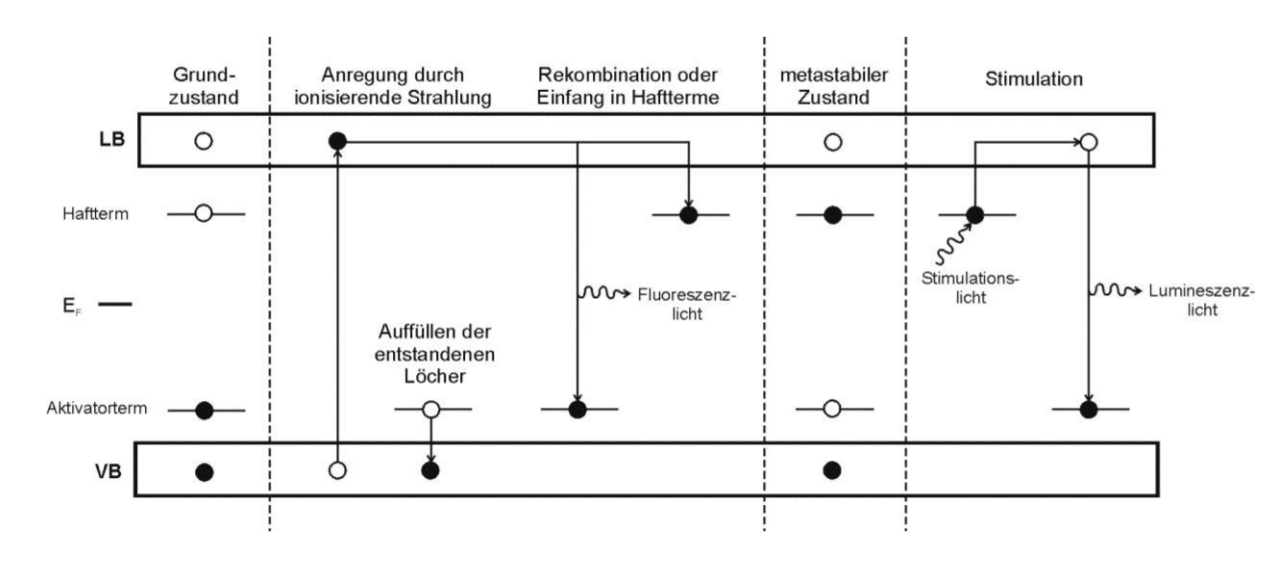
\includegraphics[width=1.1\linewidth, height=0.35\textheight]{pic/baendermodell}}
    \captionof{figure}{Schema zur optisch stimulierten Lumineszenz \cite{PA_neu}}
    \label{fig:band}
    \minipend
\end{center}

Im Grundzustand befinden sich Elektronen nur im Valenzband und den Aktivatortermen.
Regt man das System allerdings an, zum Beisiel durch ionisierende Strahlung, können einige Elektronen vom Grundzustand auf das Leitungsband oder die Hafterme springen. Aus dem Leitungsband springen sie entweder direkt un den Grundzustand, wobei sie Licht emittieren, oder fallen zunächst auf den metastabilen Zustand im Haftterm, der die Elektronen einige Zeit speichert.
Fällt nun Licht mit einer speziellen Wellenlänge auf das zuvor bestrahlte Material, springen die Elektronen aus den Hafttermen in das Leitungsband und fallen von dort meist in den Grundzustand, wobei sie Licht emittieren. \cite{PA_alt}

\subsection{BeO$max$-Funktionsprinzip}
Wir benutzen hier passive Sonden aus Berylliumoxid als Leuchtstoff. Diese Verbindung hat eine effektive Ordnungszahl von 7,13, was eine hohe Ähnlichkeit zu menschlichem Gewebe (Weichteile: 7,42, Knochen: 10) darstellt und deshalb ähnliche Absorptionseigenschaften besitzt.
Man bestrahlt die Sonden für ein zuvor berechnetes Zeitintervall. Danach sollte eine Abklingzeit von ca. 15 Minuten eingehalten werden, ehe die Sonden belichtet und ausgelesen werden. Damit wird ein Rauschen vermieden und sichergestellt, dass nur die in den Hafttermen gespeicherten Elektronen eine Rolle bei der Erzeugung des Lumineszenzlichtes spielen, bevor die Haftterme optisch angeregt werden.\\
Die passiven Sensoren haben jeder für sich ein spezifisches Ansprechvermögen, welches aus einem Signal vor der Bestrahlung, sowie nach der Bestrahlung und einer bekannten Referenzdosis bestimmt werden kann. Das Signal aus der Nullmessung ändert sich nach jeder optischen Stimulation und muss von Chip zu Chip und Messung zu Messung immer neu bestimmt werden. Damit berechnet sich das Ansprechvermögen folgendermaßen:

\begin{equation} \label{eq:ansprechvermoegen}
    \epsilon = \frac{LS_R - LS_{R,0}}{D_R}
\end{equation}
\ \\
Dabei beschreiben LS$_R$ das Lichtsignal aus der Messung bekannter Dosis, LS$_{R,0}$ das Nullsignal und D$_R$ die Referenzdosis.
Nachfolgende Gleichung beschreibt die Errechnung der Dosis aus den Lichtsignalen der Nullmessung, der Messung nach der Bestrahlung und dem Ansprechvermögen: \cite{PA_alt}
\begin{equation}
    D = \frac{LS - LS_0}{\epsilon}
\end{equation}		% Physikalischer Hintergrund
\section{Durchführung}
\subsection{Strahlenschutzkontrollmessungen}
Im Ersten Arbeitsschritt haben wir die Dosen an verschiedenen Stellen im Versuchsraum vermessen. Dabei ist zu beachten, dass das verwendete Dosimeter Messwerte über einen bestimmten Zeitraum (ca. 30 Sekunden) mittelt. Außerdem handelt es sich um die Dosen, welche am morgen zum Arbeitsbeginn gemessen wurden. %\ref{dft:Arbeitsplatz}
Im Zweiten Schritt haben wir mittels vier der BeO-Sonden, die von der Betreuerin am 21.10.2015 um 16:30 Uhr im Raum verteilt deponiert wurden, am Nachmittag des Versuchstages (23.10.15) um 15 Uhr ausgelesen.  %\ref{dft:BeOSonden} \\

	\begin{center}	

					\begin{tabular}{l|c|c|c}
								\textbf{Ort} & \textbf{\.D} [Sv/s] & \textbf{D} [mSv]  & \textbf{t$_{max}$} [h/d]\\ 
						\hline  Arbeitsplatz (vor PC) & 0,15  & 1,31   & \\ 
								50cm hinter Quelle    & 0,77  & 6,75   & \\ 
								50cm rechts der Quelle& 2,28  &        &\\ 
								50cm links der Quelle & 2,41  &        &\\ 
								50cm vor der Quelle   & 6,34  & 55.53  & \\ 
								8cm hinter der Quelle & 5,20  &        &\\ 
								8cm vor der Quelle    & 61,20 & 536,11 & \\
						\hline  50cm hinter Quelle    & 1,06  & 9,29   & \\
								50cm rechts der Quelle& 2,68  &        &\\ 
								50cm links der Quelle & 3,22  &        &\\
					\end{tabular}	
	
					\begin{tabular}{c|c|c|c}
								\textbf{Ort} & \textbf{BeO-Nr.} & \textbf{LS} [mVs] & \textbf{D} [mGy] \\
						\hline  \"{}Mitfahrer vor Quelle\" & 003337 & 14,19 & 0,5028 \\
								Auf Steckerleiste:         &        &       &        \\
								 \ \ 1,8m vor Quelle       & 003353 & 1,73  & 0,0587 \\
								 \ \ neben Quelle          & 003350 & 1,14  & 0,0437 \\
								 \ \ hinter Quelle         & 003376 & 0,19  & 0,0066 \\
						
					\end{tabular}
	\end{center}
	
Die BeO-Nummer ist die Identifikationsnummer des Sensors. Dadurch lassen sich alle Daten nochmals zurückverfolgen, da sich die Auswertesoftware die Nummern und die Verwendung der Sensoren merkt. LS bedeutet hier das gemessene Lichtsignal.
		
\subsection{Winkelabhängigkeit einer Ionisationskammer} \label{sec:Ionkammer}

Nun wenden wir uns der Messungen bezüglich der Winkelabhängigkeit der Ionisationskammer zu. Es handelt sich um eine ... Ionisationskammer. Die Messung startet bei 180\textdegree. Eine Messung dauert jeweils 60 Sekunden.

	\begin{center}
		\begin{tabular}{c|c|c|c|c}
				\textbf{$\alpha$} [\textdegree] & \textbf{d} [m] & \textbf{D$_0$} [$\mu$Gy] & \textbf{\.D$_0$} [$\mu$Gy/s] & \textbf{\.D} [$\mu$ Gy/s] \\ 
		\hline	180 & 0,50 & 18,29 & 0,304 & 0,308 \\ 
				150 & 0,50 & 18,26 & 0,304 & 0,308 \\ 
				120 & 0,50 & 17,94 & 0,299 & 0,303 \\ 
				90  & 0,50 & 17,66 & 0,294 & 0,297 \\ 
				60  & 0,50 & 17,49 & 0,292 & 0,295 \\ 
				30  & 0,50 & 17,19 & 0,287 & 0,290 \\ 
				0   & 0,50 & 17,24 & 0,288 & 0,291 \\ 
				330 & 0,50 & 17,38 & 0,290 & 0,293 \\ 
				300 & 0,50 & 17,52 & 0,292 & 0,295 \\ 
				270 & 0,50 & 17,81 & 0,297 & 0,300 \\ 
				240 & 0,50 & 18,13 & 0,302 & 0,306 \\ 
			    210 & 0,50 & 18,26 & 0,305 & 0,309 \\ 
		\hline	180 & 0,50 & 18,39 & 0,306 & 0,310 \\ 
		\end{tabular} 
	\end{center}
				

\subsection{Abschätzung der Dosisleistung für $\gamma$-Strahler}

Als nächstes widmeten wir uns der Messung der Dosis in verschiedenen Abständen. Dieses Mal verwendeten wir das BeO$max$-System. Wir verwenden immer vier der Beo-Chips in einer nahezu quadratischen Anordnung zwischen zwei verschieden dicken Plexiglas-Platten. Die dickere Platte zeigt stets von der Quelle weg.
Die BeO's müssen immer mit etwa $\Delta D = 120\ \mu$Gy bestrahlt werden, was bei verschiedenen Abständen $d$ zu verschiedenen Messzeitintervallen führt. Unter Verwendung von (\ref{eq:dosisleistung}) und (\ref{eq:aktivitaet}) erhalten wir als Abschätzung für die Bestrahlzeit:
\begin{equation}
		\Delta t 	= \frac{d^2 \cdot \Delta D}{A(t) \cdot \Gamma} 
					= 2^{\frac{t}{T_{1/2}}} \cdot \frac{d^2 \cdot \Delta D}{A_0 \cdot \Gamma} 
\end{equation}

\begin{table}
	\begin{center}
		\begin{tabular}{c|c}
				   \textbf{d} [m] & \textbf{$\Delta$t} [min] \\ 
		\hline     0,2 &  0,78 \\ 
				   0,3 &  1,76 \\ 
				   0,4 &  3,12 \\ 
				   0,5 &  4,88 \\ 
				   0,6 &  7,03 \\ 
				   0,7 &  9,56 \\ 
				   0,8 & 12,49 \\ 
				   0,9 & 15,81 \\ 
				   1,0 & 19.51 \\  
		\end{tabular} 
	\end{center}
\end{table}

\subsection{Dosismessung mit BeO$max$ und Abstandsquadratsgesetz}
Zunächst führen wir eine Kalibrationsmessung durch, um das Ansprechvermögen $\epsilon = (LS - LS_0)/D_{ref}$ zu bestimmen.In Abschnitt \ref{sec:Ionkammer} haben wir dafür die Dosisleistung bei $d=0,5\ m$ und $\alpha = 180$ \textdegree  mit $\dot{D}_{ref} = (0,309 \pm 0.001)\mu Gy /s$ bestimmt. Es ergibt sich durch die längere Messzeit von $\Delta t = 292,8\ s$ eine Dosis von $D_{ref} = \dot{D}_{ref} \cdot \Delta t = (90,5 \pm 0,4)\mu Gy$. Wobei ein systematischer Fehler bei der Zeitmessung von $\Delta(\Delta t) = 0,5s$ als Reaktionszeit angenommen wurde. Wir wiederholen nun die Messung mit dem Beo\textit{max}-System und bestimmen das Ansprechvermögen:\\
	\begin{center}	
		\begin{tabular}{c|c|c|c|c}
					\textbf{d} [m] & BeO-Nr. & \textbf{LS$_0$} [mVs] & \textbf{LS} [mVs] & \textbf{$\epsilon$} [$\frac{mVs}{\mu Gy}$] \\
			\hline  
								& 003305 & 0,66 & 2,84 & 0.024\\
						0,5		& 003398 & 0,85 & 3,68 & 0.031\\
								& 003372 & 0,77 & 3,34 & 0,028\\
								& 003312 & 0,81 & 3,18 & 0,026\\								
		\end{tabular}
	\end{center}

Damit können wir nun das gemessene Lichtsignal für alle unbekannten Dosen umrechnen. Dies sei hier examplarisch für die Messung bei $d=0,6\ m$ vorgeführt:
	\begin{center}	
		\begin{tabular}{c|c|c|c|c}
					\textbf{d} [m] & BeO-Nr. & \textbf{LS$_0$} [mVs] & \textbf{LS} [mVs] & \textbf{$\epsilon$} [$\frac{mVs}{\mu Gy}$] \\
			\hline  
								& 003305 & 0,66 & 2,84 & 0.024\\
						0,6		& 003398 & 0,85 & 3,68 & 0.031\\
								& 003372 & 0,77 & 3,34 & 0,028\\
								& 003312 & 0,81 & 3,18 & 0,026\\
								
		\end{tabular}
	\end{center}
	
%\begin{table}
	\begin{center}	
		\begin{tabular}{c|c|c|c|c}
					\textbf{d} [m] & BeO-Nr. & \textbf{LS$_0$} [mVs] & \textbf{LS} [mVs] & \textbf{D} [mGy] \\
			\hline  
								& 003305 & 0,65 & 1,99 & 0,0853\\
						0,3		& 003398 & 0,86 & 2,52 & 0,0863\\
								& 003372 & 0,79 & 2,28 & 0,0850\\
								& 003312 & 0,84 & 2,09 & 0,0846\\
			\hline  
								& 003302 & 0,93 & 2,09 & 0,0883\\
						0,4		& 003332 & 0,70 & 2,59 & 0,0899\\
								& 003395 & 1,04 & 2,09 & 0,0870\\
								& 003325 & 2,16 & 2,99 & 0,1415\\
			\hline  
								& 003312 & 0,82 & 2,48 & 0,1005\\
						0,7		& 003305 & 0,69 & 2,36 & 0,1008\\
								& 003398 & 0,88 & 3,00 & 0,1025\\
								& 003372 & 0,78 & 2,69 & 0,1002\\
			\hline  
								& 003397 & 0,66 & 2,36 & 0,1011\\
						0,8		& 003388 & 0,72 & 2,73 & 0,1025\\
								& 003364 & 0,74 & 2,39 & 0,1078\\
								& 003338 & 0,61 & 2,70 & 0,1004\\
			\hline  
								& 003325 & 2,18 & 2,15 & 0,1019\\
						0,905   & 003395 & 1,05 & 2,38 & 0,0988\\
								& 003332 & 0,69 & 3,05 & 0,1056\\
								& 003302 & 0,91 & 2,50 & 0,1056\\
			\hline  
								& 003372 & 0,80 & 2,71 & 0,1010\\
						1,0		& 003312 & 0,82 & 2,57 & 0,1038\\
								& 003398 & 0,86 & 3,08 & 0,1051\\
								& 003305 & 0,67 & 1,83 & 0,0785\\
								
		\end{tabular}
	\end{center}
%\end{table}

\subsection{Winkelabhängigkeit der kollimierten Quelle}

Zuletzt interessiert uns die Strahlaufweitung unserer Quelle. Dafür nahmen acht BeO-Sonden, die wir nebeneinander in einer Reihe auf die 16cm breite Plexiglas-Halterung legten. Die Sonden diesmal nicht zentriert, sondern von Zentrum rechtsseitig versetzt worden. Der Abstand zum Sensor um Zentrum des Strahls beträgt $d = 0,3$m. Daraus ergibt sich eine ungefähre Bestrahldauer von $\Delta t = 5$min. Die Zeit ist größer als bei den Abstandsmessungen zuvor, da sich die Abstände mit wachsendem Winkel verändert.

	\begin{center}
		\begin{tabular}{c|c|c|c|c}
				\textbf{BeO-Nr.}& \textbf{s} [cm] & \textbf{LS$_0$} [mVs] & \textbf{LS} [mVs] & \textbf{D} [mGy] \\
		 \hline 003338 &  1 & 0,62 & 6,17 & 0,2289 \\
				003302 &  3 & 0,92 & 5,43 & 0,2292 \\
				003337 &  5 & 0,48 & 6,36 & 0,2252 \\
				003364 &  7 & 0,74 & 4,98 & 0,2250 \\
				003353 &  9 & 0,44 & 5,10 & 0,1731 \\
				003388 & 11	& 0,68 & 2,15 & 0,0808 \\
				003332 & 13 & 0,73 & 1,37 & 0,0475 \\
				003376 & 15 & 0,59 & 0,74 & 0,0260 \\
		\end{tabular}
	\end{center} 
			% Durchführung
\section{Auswertung}

\subsection{Strahlenschutzmessung}

In Aufgabe 1 nahmen wir Messungen bezüglich des Strahlenschutzes vor. Dazu verwendeten wir ein mobiles Dosimeter und nahmen die aus Tabelle \ref{dft:Arbeitsplatz} bekannten Messdaten an verschiedenen Orten auf. Zur besseren Verdeutlichung, wo wir gemessen haben, folgt eine Skizze des Labors.

\vspace{5mm}

\begin{center}
    \minipanf    
        \makebox[\textwidth]{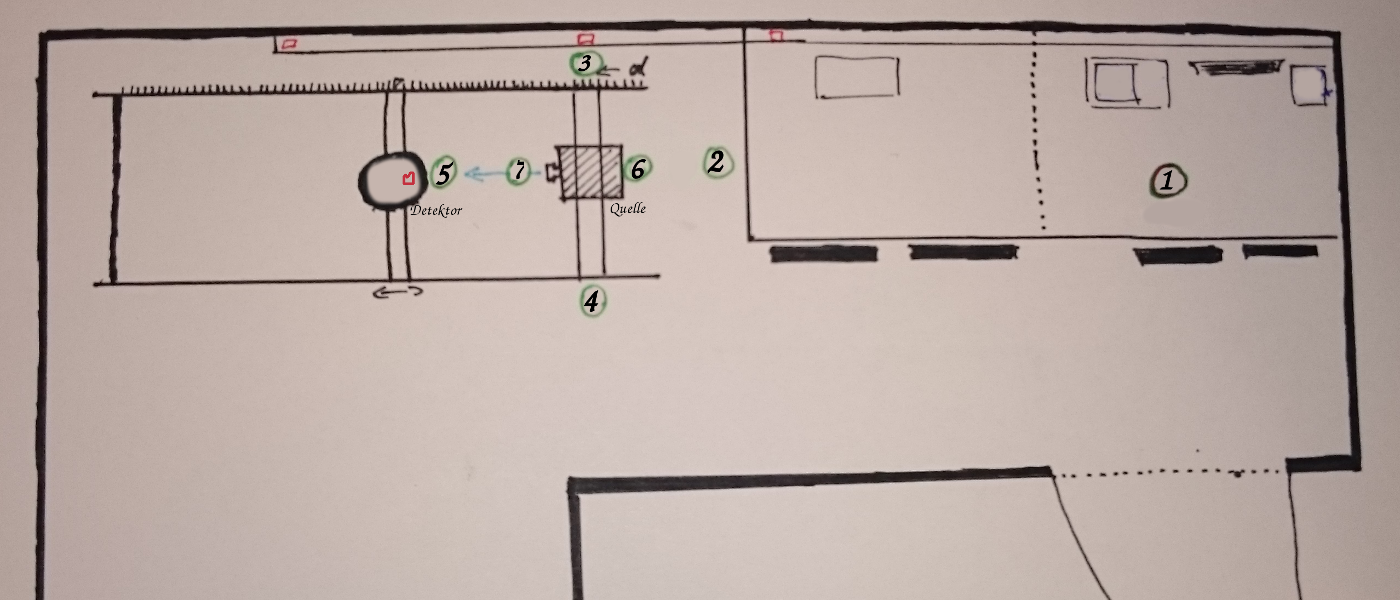
\includegraphics[width=1.4\linewidth, height=0.4\textheight]{pic/skizze}}
        \captionof{figure}{Raumskizze zu Messorten (nicht maßstabsgerecht)\\ 
                            \textbf{1:} Arbeitsplatz, \textbf{2:} 50cm hinter Quelle, \textbf{3:} 50cm rechts der Quelle, \textbf{4:} 50cm links, \textbf{5:} 50cm davor, \textbf{6:} 8cm dahinter, \textbf{7:} 8cm davor}
        \label{fig:skizze}
    \minipend
\end{center}

\vspace{5mm}

Die roten Kästchen im Bild bezeichnen die vier Punkte, an denen die BeO-Detektoren lagen. Die oberen drei liegen auf einer Steckerleiste, ca. 40cm unterhalb der Quelle. Das Kästchen bei \textbf{5} bezeichnet den \textquotedblleft Mitfahrer \textquotedblright.

\subsubsection{Strahlungswerte im Labor am Anfang des Versuchstages}

Schauen wir uns nun interessante Orte an. Tabelle \ref{dft:Arbeitsplatz} zeigt deutlich, dass am PC-Arbeitsplatz kein Risiko besteht, die 6mSv, die ein Praktikant oder Auszubildender im Jahr nicht überschreiten darf, zu erreichen. Nähert man sich der Quelle auf 50cm an und bleibt dahinter stehen, so verringert sich offenbar die maximale Aufenthaltsdauer pro Tag. Offenbar ist ein achtstündiger Arbeitstag noch immer in der Maximaldauer von 21 Stunden enthalten. \\
Jetzt wird es interessanter. Links und rechts von der Quelle, scheint die Abschirmung des Kollimators nicht mehr so stark wie hinter der Quelle. Ein Arbeitstag darf von einem Praktikanten also nicht daneben verbracht werden, sondern, unter Berücksichtigung der Fehler, die man während der Messung durch Zittrigkeit erzeugt, höchsten 7 Stunden - pro Tag, 7 Tage die Woche. 
In der Strahlrichtung vor der Quelle misst man erwartungsgemäß deutlich höhere Dosen, die die maximale Verweildauer pro Tag minimieren. 8cm vor der verschlossenen Kollimatoröffnung sollte man sich als Student möglichst weniger als 20 Minuten aufhalten.\\
Deutlich wird auch, dass die Belastung durch Strahlung überall um die Quelle größer wird, wenn man den Kollimatorverschluss öffnet. So haben wir hinter dem Kollimator zwar immer noch fast zwei Arbeitstage, um die Eintagesagesdosis zu erreichen, verlieren aber in Zahlen sechst Stunden an Aufenthaltsdauer. \\
Dabei ist zu beachten, dass die Tagesdosis den ganzen Tag betrifft, also 24 Stunden.
Die Maximaldauer ergibt sich aus der durchschnittlichen Tagesdosis folgendermaßen:

\begin{equation*}
    t_{max} = \frac{0,0164 mSv}{\dot D} 
\end{equation*}
\ \\
Dabei trägt \.D die Einheit mSv/h\\

Bezüglich der Messergegbnisse kann man noch weitere Fehlerquellen erwähnen. Das verwendete Dosimeter  ist nicht nur einer Unsicherheit durch den Haltenden ausgesetzt, sondern wurde auch bemerkt, dass zu verschiedenen Zeitpunkten die Messwerte sprungartig in die Höhe schnellten und sich nach ca. zwei Minuten senkten, was in etwa der Zeit für die Mittelung des Gerätes entspricht.

\subsubsection{Strahlendosis im Labor über 2 Tage}
Nun schauen wir uns Tabelle \ref{dft:Raum} an. Hier wurden Daten über fast zwei Tage gesammelt. Man sieht 
deutlich, dass der Mitfahrer, welcher am Versuchstag immer schwankenden Werten ausgesetzt war, eine Dosis von 
etwa 0,5mSv gemessen hat. Dies entspricht etwa der Hälfte von dem, was eine Standardperson in einem Jahr an 
künstlicher Strahlenzufuhr erfahren darf. Fraglich ist allerdings, ob dieser Wert nicht ein Ergebnis von Störungen, 
die andere Experimente verursacht haben, ist, da auch mit dem tragbaren Dosimeter zwischenzeitlich einzelne Peaks gemessen wurden.
Man erkennt allerdings gut, dass der BeO-Sensor, der hinter der Quelle lag, eine deutlich geringere Strahlendosis maß als jene, die auf der Steckerleiste 1,8m vor und auf der Steckerleiste neben der Quelle lagen. Dies bestätigt die Vermutung, die Abschirmung hinter der Quelle sei stärker als jene an den Seiten.

\subsection{Winkelabhängigkeit einer Ionisationskammer}		% Auswertung
\begin{thebibliography}{99}
\bibitem [01] {PA_alt} A.Jahn: Dosimetrie. Dresden,03/2008 
\bibitem [02] {PA_neu} A.Jahn, C. Müller: Versuchsanleitung Grundpraktikum Dosimetrie. Dresden,03/2015
\bibitem [03] {PA_RM1} PD Dr. J. Henniger; Dr. R. Schwierz; F. Hartung: Radiometrie 1 - Geiger-Müller-Zählrohr. Dresden,03/2015

\end{thebibliography}

\end{document}
